\documentclass[12pt,a5paper]{article}
\usepackage{amsmath,amsfonts,amsthm}
\usepackage[fleqn,tbtags]{mathtools}

\usepackage{courier}
\usepackage{fancyhdr} % Custom headers and footers
\usepackage{graphicx}
\usepackage{listings}
\usepackage{parskip}
\usepackage{tikz}
\usetikzlibrary{shapes,backgrounds}


\usepackage[T1]{fontenc}
\usepackage[bitstream-charter]{mathdesign}

\usepackage{titlesec} % www.ctan.org/tex-archive/macros/latex/contrib/titlesec/titlesec.pdf

% Below "\section" can be replaced with "\subsection" and "\subsubsection"
% in order to customize the corresponding headings
\titleformat{\section}[hang]{
    \usefont{T1}{bch}{b}{n}\selectfont} % "bch" - Bitstream Charter, "b" - bold
    {} % label
    {0em} % horizontal separation between label and title body
    {\Large} % code preceding the title
    [] % optional code following the title body

\setcounter{secnumdepth}{0}
\DeclareGraphicsExtensions{.pdf,.png,.jpg}

\pagestyle{fancy}
\lhead{\usefont{T1}{bch}{b}{n} Math 542 - Modern Algebra II}
\rhead{\usefont{T1}{bch}{b}{n} University of Wisconsin-Madison}


\title{\usefont{T1}{bch}{b}{n} Math 542 - HW1}         % used by \maketitle
\author{Taylor Lee}      % used by \maketitle                    % used by \maketitle


\begin{document}
\maketitle                      % automatic title!

\lstset{breaklines=true}

\setcounter{secnumdepth}{0}

\section*{Problem 1}
There are $6!$ ways to arrange six digits. If we divide this by $3!$ to remove the repeated cases for the three ones, and also divide by $2!$ for the repeated cases of the twos, we find that there are
\[
\frac{6!}{2! \cdot 3!} = 60
\]
ways to arrange this list.

As given in the book there are $C(5 + 4 -1,4)$ ways to select four bottles of wine from an infinite selection of five types. This value is equal to $70$.

\section*{Problem 2}
By starting at one vertex, we can draw a line to the five other points. Moving clockwise, to the next vertex, we now see that there are only four remaining vertices that we can draw a line to. Continuing aroung the hexagon clockwise, we see that this trend continues, and so the total number of lines that we have drawn is:
\[
5 + 4 + 3 + 2 + 1 = 15
\] 

On further examinaiton of our hexagon, we can see that there are a total of twenty triangles that have formed.


\section*{Problem 3}
\subsection*{Part A}
After a triangular sketch which I could not recreate, I found the answer to be
\[
10! + \frac{10!}{2!} + \frac{10!}{4!} + \frac{10!}{6!} + \frac{10!}{8!}
\]
In a few words, there are 9 ways a natural number can be represented with one digit. For two digits, we had the count at ten permute two, minus the 9 from the one digit case. This patteren continued all the way up to ten digits, and summing all ten rows together, one finds that terms which first emerge on an odd number of digits are canceled out, as they will come in offsetting pairs throughout the remainder of the table. This is similar the the argument used in part B.


\subsection*{Part B}
We first start with the obvious: there are only two numbers with two digits including eight and nine only once. For three digits, we have $8 \cdot 3! - 2$, as because there are six possible ways our three numbers can be organized, and eight numbers we can insert in as our third. We also must compensate for the numbers which lead by zero, and hence subtract the number of our two digit numbers, as these have a clear correspondence. Next, for four digits, we have $8 \cdot 8 \cdot 4! -  8 \cdot 3! + 2$, the same reasoning follows. Hence, by adding these three numbers together, we are left with:
\[
8 \cdot 8 \cdot 4! + 2 = 1538
\]


\section*{Problem 1}

Let us first realize our three given pieces of information with Venn diagrams. Sixty percent of all bills pass the House:

\begin{center}
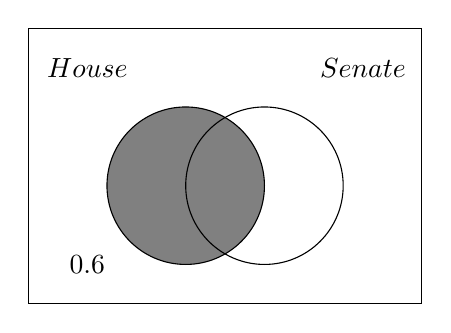
\begin{tikzpicture}
\draw (-2,-1.5) rectangle (3,2);
\fill[gray] (0,0) circle (1cm);
\draw (0,0) circle (1cm);
\draw (1,0) circle (1cm);
\draw (-1.25,1.5) node {$House$};
\draw (2.25,1.5) node {$Senate$};
\draw (-1.25,-1.0) node {$0.6$};
\end{tikzpicture}
\end{center}

Eighty percent of our bills pass the Senate:

\begin{center}
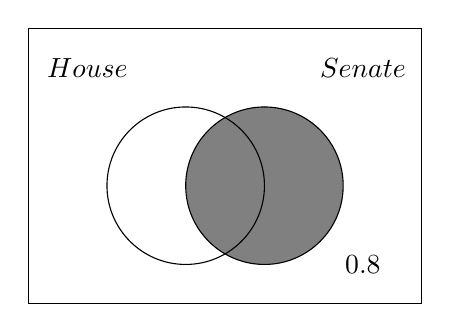
\begin{tikzpicture}
\draw (-2,-1.5) rectangle (3,2);
\fill[gray] (1,0) circle (1cm);
\draw (0,0) circle (1cm);
\draw (1,0) circle (1cm);
\draw (-1.25,1.5) node {$House$};
\draw (2.25,1.5) node {$Senate$};
\draw (2.25,-1.0) node {$0.8$};
\end{tikzpicture}
\end{center}

And lastly, Ninety percent pass one of the two houses, which is the union of the two events:
\begin{center}
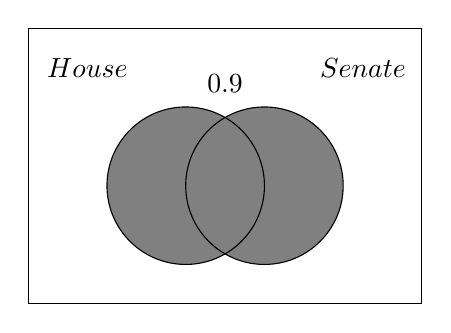
\begin{tikzpicture}
\draw (-2,-1.5) rectangle (3,2);
\fill[gray] (0,0) circle (1cm);
\fill[gray] (1,0) circle (1cm);
\draw (0,0) circle (1cm);
\draw (1,0) circle (1cm);
\draw (-1.25,1.5) node {$House$};
\draw (2.25,1.5) node {$Senate$};
\draw (.5,1.3) node {$0.9$};
\end{tikzpicture}
\end{center}

With the formula for the probability of the union of events, we can see that our intersection is equal to $.8+.6-.9 = .5$.

\begin{center}
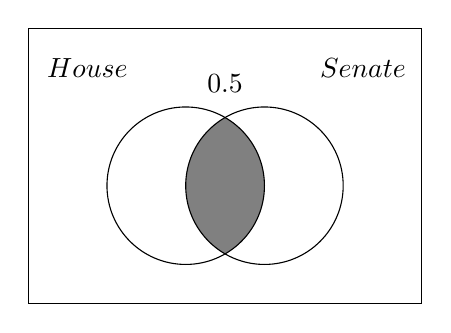
\begin{tikzpicture}
\draw (-2,-1.5) rectangle (3,2);
\begin{scope} % start of clip scope
\clip (0,0) circle (1cm);
\fill[gray] (1,0) circle (1cm);
\end{scope} % end of clip scope
\draw (0,0) circle (1cm);
\draw (1,0) circle (1cm);
\draw (-1.25,1.5) node {$House$};
\draw (2.25,1.5) node {$Senate$};
\draw (.5,1.3) node {$0.5$};
\end{tikzpicture}
\end{center}

\section*{Problem 2}
We can easily solve this problem by first finding the probabilities that one box and two boxes will be empty, and then subtracting the sum of these two results from $1$ in order to find the probability that no box will be left empty.

First, if we choose a box which is to be left empty, then we must multiply $\frac{2}{3}^6$, as this is the probability that we will place the current ball into one of the other two boxes six times in a row, followed by multiplying this number by three, as there are three different ways we can exclude a single box.

Secondly, if we choose a lone box which is to be filled with all six balls, then we must multiply $\frac{1}{3}^6$, as this is the probability that we will place the current ball into the designated box six times in a row, followed by multiplying this number by three, as there are three different ways we can exclude two boxes.

Subtracting this sum from $1$, we get:

\[
1 - \frac{2^6}{3^5} - \frac{1}{3^5} = 1 - \frac{64}{243} - \frac{1}{243} = \frac{178}{243} = .7325102881
\]

\section*{Problem 3}

Let us suppose that our left urn has two red and three blue balls, and that our right urn has four red and four blue balls. If we first take a ball from the left urn to the left, our probability of drawing red is as follows.

\[
B \rightarrow = \frac{3}{5} \cdot \frac{4}{9}, R \rightarrow = \frac{2}{5} \cdot \frac{5}{9}.
\]

And likewise if we were to take from the right urn and place it into the left:

\[
B \leftarrow = \frac{1}{2} \cdot \frac{1}{3}, R \leftarrow = \frac{1}{2} \cdot \frac{1}{2}.
\]

There is an equal chance of either of these two lines taking place, and we can sum the two probabilities on each line together in order to find the chances of drawing red if such a line were to occur. Hence:

\[
.5 \left( \frac{12}{45} + \frac{10}{45} \right) + .5 \left( \frac{2}{12} + \frac{3}{12} \right) = \frac{11}{45} + \frac{5}{24} = .4577777778
\]


\section*{Problem 4}
We begin by creating a table of all possible outcomes.
\begin{tabular}{ c || c | c | c | c | c | c }
& 1 & 2 & 3 & 4 & 5 & 6 \\
\hline
\hline
1 & 2 & 3 & 4 & 5 & 6 & 7 \\
\hline
2 & 3 & 4 & 5 & 6 & 7 & 8 \\
\hline
3 & 4 & 5 & 6 & 7 & 8 & 9 \\
\hline
4 & 5 & 6 & 7 & 8 & 9 & 10 \\
\hline
5 & 6 & 7 & 8 & 9 & 10 & 11 \\
\hline
6 & 7 & 8 & 9 & 10 & 11 & 12 \\
\end{tabular}

We now create a table with the probabilities of rolling each of the sums:

\begin{tabular}{|c | l|}

\hline
S & p(S) \\
\hline
2 & 0.0277777777778 \\
\hline
3 & 0.0555555555556 \\
\hline
4 & 0.0833333333333 \\
\hline
5 & 0.111111111111 \\
\hline
6 & 0.138888888889 \\
\hline
7 & 0.166666666667 \\
\hline
8 & 0.138888888889 \\
\hline
9 & 0.111111111111 \\
\hline
10 & 0.0833333333333 \\
\hline
11 & 0.0555555555556 \\
\hline
12 & 0.0277777777778 \\
\hline
\end{tabular}

With a bit of artihmetic, we can find that $E(S) = 7$.



\section*{Problem 5}

\subsection*{Part A}
Since we must filp tails $k-1$ times before fliping heads on the $k-th$ times, our probability of flipping heads is:
\[
P(k) = p(1-p)^{k-1}
\]

\subsection*{Part B}
This is a good example of a geometric distribution. Our expected value for $k$ is defined with the following sum, as given in the book:

\[
\sum_{k=1}^{\infty} kp(1-p)^{k-1} = p \sum_{k=1}^{\infty} k(1-p)^{k-1} = p \frac{1}{p^2} = \frac{1}{p}
\]




\section*{Problem 6}

\subsection*{Part A}

The probability that a car is behind one of the $k$ doors is $\frac{n-1}{nk}$, since the probability that we did not choose the car initially is $\frac{n-1}{n}$, and given that this happened (That our car was not choosen initially), there is a $\frac{1}{k}$ chance that our car will be behind one of the $k$ remaining doors. Hence
\[
p_{n,k} = \frac{n-1}{nk}.
\]

\subsection*{Part B}
With a little bit of calculus, we can evaluate the limit 

$\lim_{n \rightarrow \infty} p_{n,k}$, we multiply the top and bottom of $p_{n,k}$ by $\frac{1}{n}$. Hence we get:

\[
\frac{1-\frac{1}{n}}{k} = \frac{1}{k}.
\]


\end{document}   
